\documentclass[UTF8]{ctexart}
\usepackage{cite}   %引用
\usepackage{url}    %引用网址
\usepackage{geometry}   %页边距
\usepackage{graphicx}   %图片
\usepackage{setspace}   %行间距
\usepackage{indentfirst} %首行缩进
\usepackage{amsmath}
\geometry{left=2.0cm,right=2.0cm,top=2.5cm,bottom=2.5cm}
\renewcommand{\baselinestretch}{1.5}
\setlength{\parindent}{2em} 
\begin{document}
\title{\textbf{Stereo Project Report}}
\author{赵懿-武汉大学 网络空间安全学院}
\maketitle
\section{Camera Basics}
\subsection{第一问:intrinsics, extrinsics,camera matrix}
解释这个问题首先需要解释相机拍摄真实世界物体进行的模型。
\subsubsection{模型}
对于拍摄问题存在三个坐标系\cite{CameraModels18830}:
\begin{itemize}
  \item 世界坐标系:用于表示世界中的物体(点,线,表面等)的固定坐标系,3D
  \item 相机坐标系:以摄像机中心为原点(光轴为Z轴)的坐标系,3D
  \item 底片坐标系:测量图像平面中像素位置的坐标系,位于相机底片上,2D
\end{itemize}
拍摄过程即是对真实世界的一个点进行投影变换到底片上的过程。即世界坐标系的一个点经过投影变换到底片坐标系中的一个点。我这对模型画了一个示意图(\#图是自己画的有点难看):
\begin{figure}[htp]%%图
	\centering  %插入的图片居中表示
	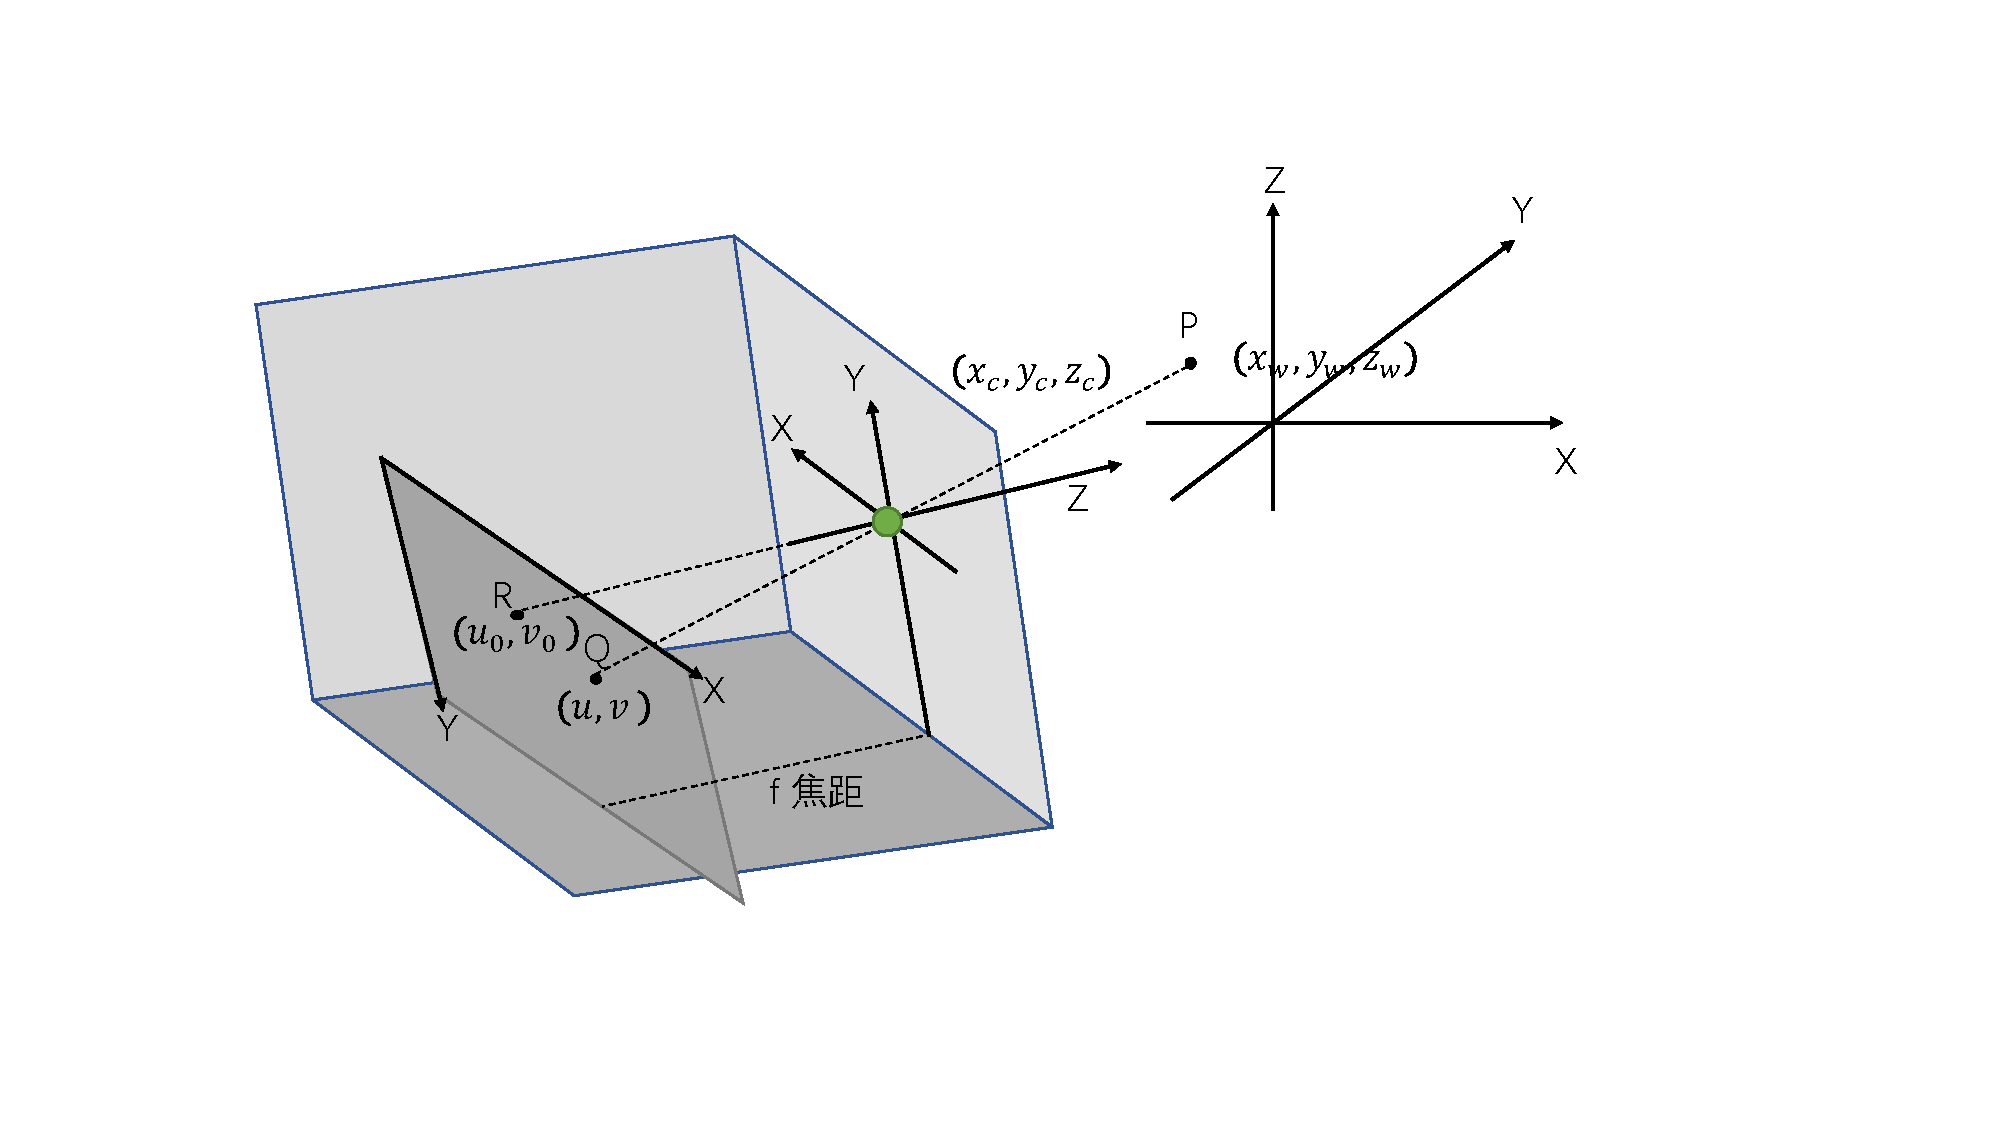
\includegraphics[width=0.5\linewidth]{./figures/model.pdf} %插入的图,包括JPG,PNG,PDF,EPS 等,放在源文件目录下
	\caption{投影模型}  %图片的名称
	\label{fig:model}   %标签,用作引用
\end{figure}\\
在我画的模型其中:点$P$值真实世界中一点;$(x_w,y_w,z_w)$:点$P$在世界坐标系中的坐标;$(x_c,y_c,z_c)$: 点$P$在相机坐标系中的坐标;点$R$:底片中心坐标,也是相机坐标系$Z$轴(光轴)和底片相交的点;点$Q$: 点$P$在底片的投影;$(u,v)$:$Q$ 在底片坐标系中的坐标;$f$为相机焦距。\\
显然从$P$到$Q$包含两个变换:
\begin{figure}[htp]%%图
	\centering  %插入的图片居中表示
	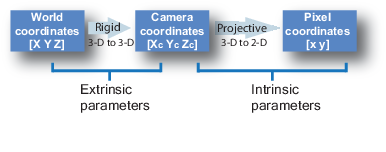
\includegraphics[width=0.8\linewidth]{./figures/calibration_coordinate_blocks.png} %插入的图,包括JPG,PNG,PDF,EPS 等,放在源文件目录下
	\caption{投影变换的坐标系变换\cite{MathWorks18830}}  %图片的名称
	\label{fig:calibration_coordinate_blocks}   %标签,用作引用
\end{figure}\\
写成矩阵形式如下:
\begin{equation}       %开始数学环境
z_c \left[ \begin{array}{c}  u \\ v \\  1 \end{array} \right] =
K \left[ \begin{array}{c|c} R & T   \end{array} \right] \left[ \begin{array}{c}   x_w \\  y_w \\  z_w \\ 1 \end{array}\right]
\end{equation}
\textbf{其中$K$为intrinsics matrix(也即是camera matrix),$[R|T]$ 为extrinsics matrix\cite{wikiCameraresectioning18830}。}
\subsubsection{Extrinsics matrix的含义}
由模型可以看出,extrinsics matrix($[R|T]$)是世界坐标点P(3D)到相机坐标点P(3D)的投影转换矩阵。真实世界点P坐标左乘$[R|T]$后得到点P在相机坐标系中的坐标值:
\begin{align}
 \left[ \begin{array}{c}  x_c \\ y_c \\  z_c \end{array} \right] &=
 \left[ \begin{array}{c|c} R & T   \end{array} \right] \left[ \begin{array}{c}   x_w \\  y_w \\  z_w \\ 1 \end{array}\right]\\
 \left[ \begin{array}{c|c} R & T   \end{array} \right] &=
\left[ \begin{array}{ccc|c}
r_{1,1} & r_{1,2} & r_{1,3} & t_1 \\
r_{2,1} & r_{2,2} & r_{2,3} & t_2 \\
r_{3,1} & r_{3,2} & r_{3,3} & t_3 \\
\end{array} \right]
\end{align}
这个变换可以理解为一个坐标系的旋转和平移,其中$R$是旋转矩阵,$T$是位移向量。由线性代数的知识可以指导,两个坐标系都是3D的,所以$R$的shape是3*3,$T$的shape是3*1。关于$R$的解释我是参考的wiki\cite{wikiRotationmatrix18830},解释得比较清楚;$T$是表示平移变换矩阵,为真实世界坐标系原点在相机坐标系中的坐标值。
\subsubsection{Intrinsics matrix的含义}
Intrinsics matrix K 是相机坐标点(3D)到底片坐标点(2D)的映射转换矩阵。即:
\begin{align}
 z_c \left[ \begin{array}{c}  u \\ v \\ 1 \end{array} \right] &=
 K \left[ \begin{array}{c}   x_c \\  y_c \\  z_c  \end{array}\right]\\
K &= \left [ \begin{array}{ c c c}
f_x & s   & x_0 \\
0  & f_y & y_0 \\
0  & 0   & 1 \\
\end{array} \right ]
\end{align}
我参考wiki\cite{Pinholecameramodel18830}看了针孔摄像机原理,参考了这篇CSDN博客\cite{CSDNJessicajiel18830}(开始一直不理解$f_x,f_y$的意义)了解了参数的意义:
\begin{figure}[htp]%%图
	\centering  %插入的图片居中表示
	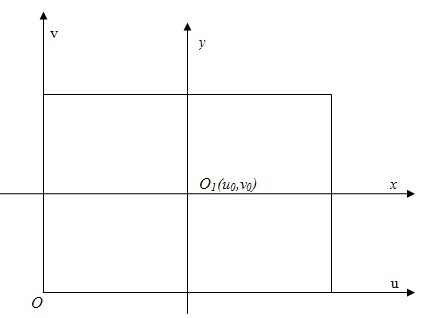
\includegraphics[width=0.5\linewidth]{./figures/twocor.jpg} %插入的图,包括JPG,PNG,PDF,EPS 等,放在源文件目录下
	\caption{底片上的两个坐标系}  %图片的名称
	\label{fig:calibration_coordinate_blocks}   %标签,用作引用
\end{figure}\\
上图是建立在相机底片平面上的两个坐标系。其中原点在左下角的$(u,v)$坐标系是像素坐标系,$u,v$单位为像素的宽$d_x$和高$d_y$;原点在中间的$(x,y)$坐标系是成像平面坐标系,$x,y$单位为物理意义的长度(毫米之类的),记$(x,y)$坐标系原点在$(u,v)$坐标系中的坐标为$(u_0,v_0)$。\\
通过\cite{Pinholecameramodel18830}针孔成像原理(相似三角形)可以推出相机坐标系中点$P(x_c,y_c,z_c)$在底片成像平面坐标系中的坐标$(x_m,y_m)$:
\begin{align}
 z_c \left[ \begin{array}{c}  x_m \\ y_m \\ 1 \end{array} \right] =
 M \left[ \begin{array}{c}   x_c \\  y_c \\  z_c  \end{array}\right], where: 
 M = \left [ \begin{array}{ c c c}
f & 0   & 0 \\
0  & f & 0 \\
0  & 0   & 1 \\
\end{array} \right ]
\end{align}
同时,可以推出成像平面坐标系中的坐标点$(x_m,y_m)$到像素坐标系点$(u,v)$的公式:
\begin{align}
z_c \left[ \begin{array}{c}  u \\ v \\ 1 \end{array} \right] =
 Q \left[ \begin{array}{c}   x_m \\  y_m \\  1  \end{array}\right], where:
Q = \left [ \begin{array}{ c c c}
\frac{1}{d_x} & 0   & u_0 \\
0  & \frac{1}{d_y} & v_0 \\
0  & 0   & 1 \\
\end{array} \right ]
\end{align}
所以相机内矩阵$K$即为:
\begin{align}
K = QM= 
\left [ \begin{array}{ c c c}
f & 0   & 0 \\
0  & f & 0 \\
0  & 0   & 1 \\
\end{array} \right ]
\left [ \begin{array}{ c c c}
\frac{1}{d_x} & 0   & u_0 \\
0  & \frac{1}{d_y} & v_0 \\
0  & 0   & 1 \\
\end{array} \right ]
=
\left [ \begin{array}{ c c c}
\frac{f}{d_x} & 0   & u_0 \\
0  & \frac{f}{d_y} & v_0 \\
0  & 0   & 1 \\
\end{array} \right ]
\end{align}
\subsection{第二问:3D到2D(自己推的)}
通过section 1.1的原理,显然:
\begin{align*}
K = \left [ \begin{array}{ c c c}
f_x & 0   & c_x \\
0  & f_y & c_y \\
0  & 0   & 1 \\
\end{array} \right ],
[R|T]=(R|t), so:
 z_c \left[ \begin{array}{c}  u \\ v \\ 1 \end{array} \right] =
 K \left[ \begin{array}{c}   X_1 \\  X_2 \\  X_3 \\ 1  \end{array}\right]
\end{align*}
$(u,v)$即为$(X_1,X_2,X_3)$在image plane上的投影点。
\subsection{第三问:2D到3D(自己推的)}
给定2D的点$(u,v)$,该点在3D相机矩阵中对应的shape是一条直线。推理如下:
设$(u,v)$在3D相机矩阵中对应的点(集)坐标为$(x,y,z)$,相机内矩阵为$K$。则有:
$$z(u,v,1)^T=K(x,y,z)^T$$
因为$K$为3D方阵,且其行列式$|K|=f_x*f_y*1>0, becuase f_x>0, f_y>0$,所以$K$的逆矩阵$K^{-1}$存在,则:
\begin{align}
(x,y,z)^T=zK^{-1}(u,v,1)^T=z(a,b,c)^T\label{equ:lineExpress}
\end{align}
现在1.给定$u,v$,2.$K$不随$u,v$变化,为确定值,则上式中$a,b,c$为确定值,$z$未知。所以在相机矩阵中,在
\begin{align}
\frac{x}{a}=\frac{y}{b}=\frac{z}{c}
\end{align}
直线上的点都满足(\ref{equ:lineExpress})式。所以,2D点$(u,v)$对应3D相机中形状$(x,y,z)$的公式为:
\begin{align}
\frac{x}{a}=\frac{y}{b}=\frac{z}{c},where:(a,b,c)^T=K^{-1}(u,v,1)
\end{align}
\#emmm,抱歉老师,我没推出来为什么$a,b,c\neq0$
\subsection{第四问:Distortion,相机畸变}
\#理解相机的畸变主要参考了这篇CSDN的博客\cite{CSDNJessicajiel18830}。\\
畸变(distortion)是对直线投影(rectilinear projection)的一种偏移。相机的畸变简单来说就是真实世界找那个一条直线投影到图片上不能保持为一条直线了。相机畸变主要包括两种类型:
\begin{description}
  \item[径向畸变] 这种畸变来自于透镜形状。对某些透镜,该现象是由于光线在远离透镜中心的地方比靠近中心的地方更加弯曲,产生“筒形”或“鱼眼”形成的。一般来讲,成像仪中心的径向畸变为0,越向边缘移动,畸变越严重。对于这种畸变,可以通过泰勒展开式矫正:
  $$
  x''=x'(1+k_1r^2+k_2r^4),
  y''=y'(1+k_1r^2+k_2r^4),
  where:r=x'^2+y'^2
  $$
  其中$(x'',y'')$是矫正后的理想(无畸变)坐标,$(x',y')$是存在畸变的真实相机坐标系找那个坐标。我对上式的理解是,由于随着$r$增大,该类型畸变越严重,所以上面的矫正方法也是$r$越大,矫正力度越大。
  \item[切向畸变] 当成像仪被粘贴在摄像机的时候,会存在一定的误差,使得图像平面和透镜不完全平行,从而产生切向畸变。也就是说,如果一个矩形被投影到成像仪上时,可能会变成一个梯形。对于这种畸变,可以以下公式来矫正:
  $$
  x''=x'+(2p_1y',p_2(r^2+2x'^2)),
  y''=y'+(2p_1x',p_2(r^2+2y'^2)),
  where:r=x'^2+y'^2
  $$
  以上公式中的符号定义与径向畸变相同。
\end{description}
同时考虑两种畸变,则纠正畸变的公式为:
\begin{align}
  x''&=x'(1+k_1r^2+k_2r^4)+(2p_1y',p_2(r^2+2x'^2))\\
  y''&=y'(1+k_1r^2+k_2r^4)+(2p_1x',p_2(r^2+2y'^2))
\end{align}
以上公式中的符号定义与径向畸变相同。
\subsection{第五问:Calibration相机标定}
像机标定主要是求出相机的内、外参数,以及畸变参数。其主要步骤是\cite{zhang2000flexible}:
\begin{enumerate}
  \item 打印一张棋盘格贴到一个平面上
  \item 移动平面或摄像机,从不同方向拍摄多张模板平面的图像
  \item 从图像中检测特征点
  \item 在不考虑畸变的情况下,估计相机内矩阵的5个参数和每幅图片的外参
  \item 用相机内矩阵和外参估计畸变参数
  \item 通过极大似然估计优化以上求出的参数
\end{enumerate}
\subsection{第六问:openCV相机标定}
#实现这个程序主要参考了\cite{opencvCameraCalibrationl18830}的官方API
实现的代码
\bibliographystyle{plain}
\bibliography{myreference}
\end{document}
